\documentclass{beamer}

\mode<presentation> {

\usetheme{Copenhagen}
\usecolortheme{seagull}
}

\usepackage{graphicx}
\DeclareGraphicsExtensions{.pdf,.png,.jpg}
\usepackage{booktabs} % Allows the use of \toprule, \midrule and \bottomrule in tables
\usepackage{mathtools}
\usepackage{multirow}
\usepackage{color, colortbl}
\usepackage{minted}

%----------------------------------------------------------------------------------------
%	TITLE PAGE
%----------------------------------------------------------------------------------------

\title[Test]{Test}

\author{Rasmus Guldborg Pedersen}

\date{June 2015}

\begin{document}

\begin{frame}
\titlepage
\end{frame}

\begin{frame}
\frametitle{Overview}
\tableofcontents
\end{frame}



\section{Q 2.5: Control-flow testing}

\begin{frame}
    \frametitle{Control-Flow Testing}
    \begin{itemize}
        \item White-box testing
        \item Control-Flow Graphs
        \item Good coverage
    \end{itemize}
\end{frame}

\begin{frame}[fragile]
    \frametitle{Example Code}
    \begin{minted}[linenos]{csharp}
int Factorial(int n) {
    int f = 1;
    if (n < 0)
    {
        // -1 indicates an error
        f = -1;
    }
    else
    {
        for (int i = 1; i < n; i++)
        {
            f *= i;
        }
    }
    return f;
}
    \end{minted}
\end{frame}

\begin{frame}
    \frametitle{Example Graph}
    \centering
    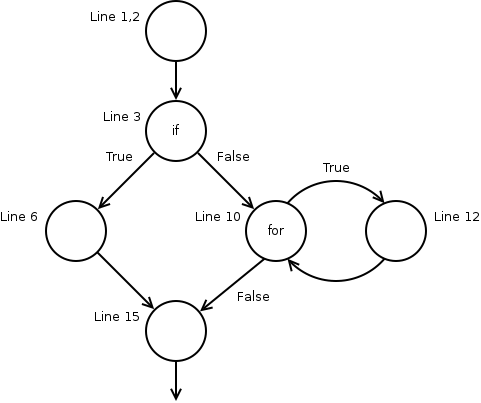
\includegraphics[scale=0.4]{state_transition.png}
\end{frame}

\begin{frame}
    \frametitle{Coverage Criteria}
    \begin{itemize}
        \item Statement Coverage
            \begin{itemize}
                \item All statements are executed
                \item Weakest
            \end{itemize}
        \item Decision Coverage
            \begin{itemize}
                \item All branches covered
                \item Stronger than statement coverage
            \end{itemize}
        \item Loop Coverage
            \begin{itemize}
                \item Loop boundary
                \item 0, 1, highest valid, lowest valid
            \end{itemize}
    \end{itemize}
\end{frame}


%------------------------------------------------

\begin{frame}
    \frametitle{The End}

    %\Huge{\centerline{The End}}
    \begin{quote}
        ``Testing shows the presence, not the absence of bugs.''
        \raggedleft{--- Edsger W. Dijkstra}
    \end{quote}
\end{frame}

%----------------------------------------------------------------------------------------

\end{document}

